\documentclass[article,latterpaper]{article}
\usepackage[utf8]{inputenc}
\usepackage{float}
\usepackage[spanish]{babel}
\usepackage{geometry}
\usepackage{url}
\usepackage{cite}
\usepackage[pdftex]{graphicx}
\usepackage{amssymb}
\usepackage{amsmath}
\usepackage{hyperref}
\usepackage{xurl}
\usepackage{caption}
\usepackage{array}
\usepackage{multirow}
\usepackage{comment}
\usepackage{fancyhdr}

\title{Proyecto final\\Solución de la ecuación de difusión con código paralelizado}
\author{}
\date{\today}

\makeatletter
\let\thetitle\@title
\let\theauthor\@author
\let\thedate\@date
\makeatother

\pagestyle{fancy}
\fancyhf{}
\rhead{\thedate}
\lhead{\thetitle}
\cfoot{\thepage}
\renewcommand{\baselinestretch}{1.5}


\begin{document}

\begin{titlepage}
  \centering
  \vspace{0.2 cm}
  
\includegraphics[scale = 0.4]{PNG_LOGOSIMBOLO CENTRAL 2 COLORES (VERDE Y GRIS)-02-02-02.png} \\
  \textsc{\Large 2023-1} \\[0.5 cm]
  \rule{\linewidth}{0.2 mm} \\[0.2 cm]
  {\LARGE \bfseries \thetitle} \\
  \rule{\linewidth}{0.2 mm} \\[2 cm]
  \begin{minipage}{0.8\textwidth}
    \raggedright
    \emph{Autor:}\\
    Kevin Cortés - kcortesr@unal.edu.co\\
    \hfill\break
    \emph{Profesor:}\\
    William Fernando Oquendo Patiño\\
  \end{minipage}  
\end{titlepage}

\newpage
\begin{center}
  \pagenumbering{Roman}
  \tableofcontents
\end{center}

\newpage
\pagenumbering{arabic}

\section{Introducción}
El proyecto realizado para el segundo módulo del curso \textbf{introducción a la computación científica de alto rendimiento} es la implementación del método de volúmenes finitos (\textit{FVM} por sus siglas en Inglés) para solucionar la ecuación de difusión en un problema de conducción de calor en una placa rectangular en estado estacionario. Adicionalmente, el código de la función de la malla y de la función de procesamiento se paralelizan haciendo uso de \textbf{OpenMP}.

Ahora bien, el flujo de trabajo llevado a cabo es:

\begin{itemize}
	\item Discretización a mano de la ecuación de difusión.
	\item Programación de la malla.
	\item Programación de las propiedades físicas y del término fuente.
	\item Programación de las condiciones de frontera.
	\item Programación de la etapa de procesamiento: La solución del sistema de ecuaciones se realizó mediante el método iterativo de Gauss - Seidel.
	\item Programación de la etapa de posprocesamiento: Obtención de las gráficas que muestran los resultados.
        \item Análisis de los resutados de las métricas paralelas.
\end{itemize}

Cada vez que se obtuvo avances los archivos y casos fueron subidos a un repositorio de \textbf{GitHub} cuyo enlace es: \url{https://github.com/KevinCortesR/Proyecto_ICCAR.git}

\subsection{Objetivos específicos}
    \begin{itemize}
        \item Utilizar la herramienta \textbf{OpenMP} con el fin de paralelizar las etapas de creación de la malla y solución del problema de interés.
        \item Obtener gráficas de \textit{speed-up} y de \textit{parallel efficiency} utilizando la librería \textbf{chrono} para medir el \textit{wall-clock time} y la función \textbf{std::clock\_t} para medir el \textit{CPU time}.
        \item Obtener gráficas del desempeño del código para diferentes grados de optimización.
    \end{itemize}

\vspace{1.5 cm}

Por otra parte, para comprobar el funcionamiento de los códigos realizados se hizo la implementación de un caso con solución analítica. Una vez comprobados, se solucionó el problema de interés y se analizaron los resultados.

\section{Problema de interés}
Se tiene una placa plana como se muestra a continuación:

\begin{figure}[H]
    \centering
    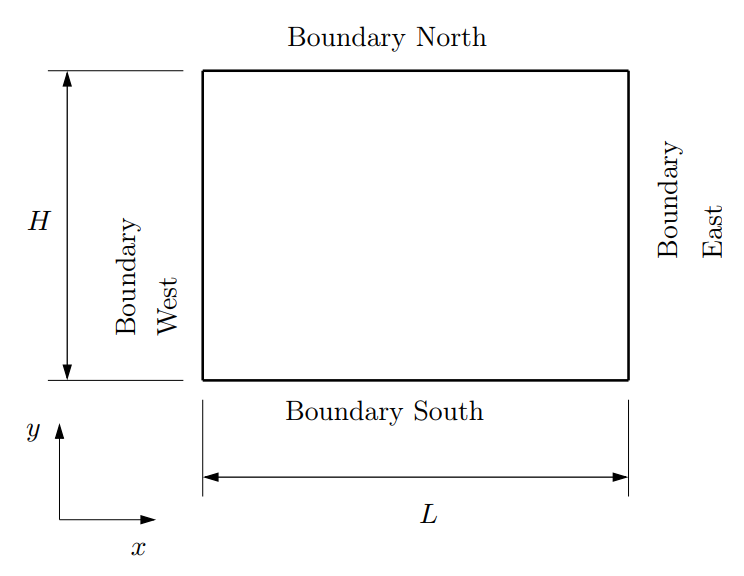
\includegraphics[scale=0.3]{Prob_CFD1.png}
    \caption{ \centering{Geometría de la placa: $L=3$ m y $H=2$ m}}
    \label{Dom_cp}
\end{figure}

Para esta placa se tienen las siguientes condiciones de frontera, conductividad témica y término fuente:

$$
\begin{array}{|cc|}
    \hline \text { Frontera } & \text { Condición } \\
    \hline \text { Norte } & \frac{\partial T}{\partial y}=0 \text { (adiabatica) } \\
    \text { Sur } & T=-5+20\left(\frac{x}{L}\right)^2+20 \sin \left(\frac{4 \pi x}{L}\right) \\
    \text { Oeste } & T=-5^{\circ} \mathrm{C} \\
    \text { Este } & T=15^{\circ} \mathrm{C} \\
    \hline \text { Conduct. } & \kappa=2\left(2.5-\frac{x}{L}\right) \mathrm{W} / \mathrm{m} \cdot{ }^{\circ} \mathrm{C} \\
    \text { Fuente } & B=100 \\
    \hline
\end{array}
$$

La ecuación de difusión que rige el problema es la siguiente:

\begin{equation}
    0 = \frac{\partial}{\partial x} \left( \kappa \frac{\partial T}{\partial x}  \right) +  \frac{\partial}{\partial y} \left( \kappa \frac{\partial T}{\partial y}  \right) +B
    \label{Ec_difusion}      
\end{equation}

\subsection{Discretización}

A continuación, se muestra la discretización la ecuación \eqref{Ec_difusion}; aunque se deja en la forma genérica, es decir en términos de $\phi$ y $\Gamma$ . En primera instancia, al integrar sobre el volumen se obtuvo:

\begin{equation}
    0 = \int_V \left[ \frac{\partial}{\partial x} \left( \Gamma \frac{\partial \phi}{\partial x}  \right) +  \frac{\partial}{\partial y} \left( \Gamma \frac{\partial \phi}{\partial y}  \right) \right] dV + \int_V B dV
    \label{int_V_eq1}
\end{equation}

Para evitar lidiar con la segunda derivada, se hizo uso del teorema de la divergencia de Gauss para un campo vectorial arbitrario $C$:

\begin{equation}
    \int_V (\nabla \cdot C) \: dV = \int_S (C \cdot \hat{n}) \: dS
\end{equation}

Aplicando el teorema a la ecuación \eqref{int_V_eq1} y suponiendo un término fuente $B$ constante se tuvo:

\begin{equation}
    0 = \int_S \left[ \Gamma \frac{\partial \phi}{\partial x} \hat{n}_x + \Gamma \frac{\partial \phi}{\partial y} \hat{n}_y  \right] dS + B V 
    \label{int_S_eq1}
\end{equation}

Para una celda interior $P$, los vectores normales en función de sus celdas vecinas al norte, sur, este y oeste tomaron valores como se muestra en la siguiente figura:

\begin{figure}[H]
    \centering
    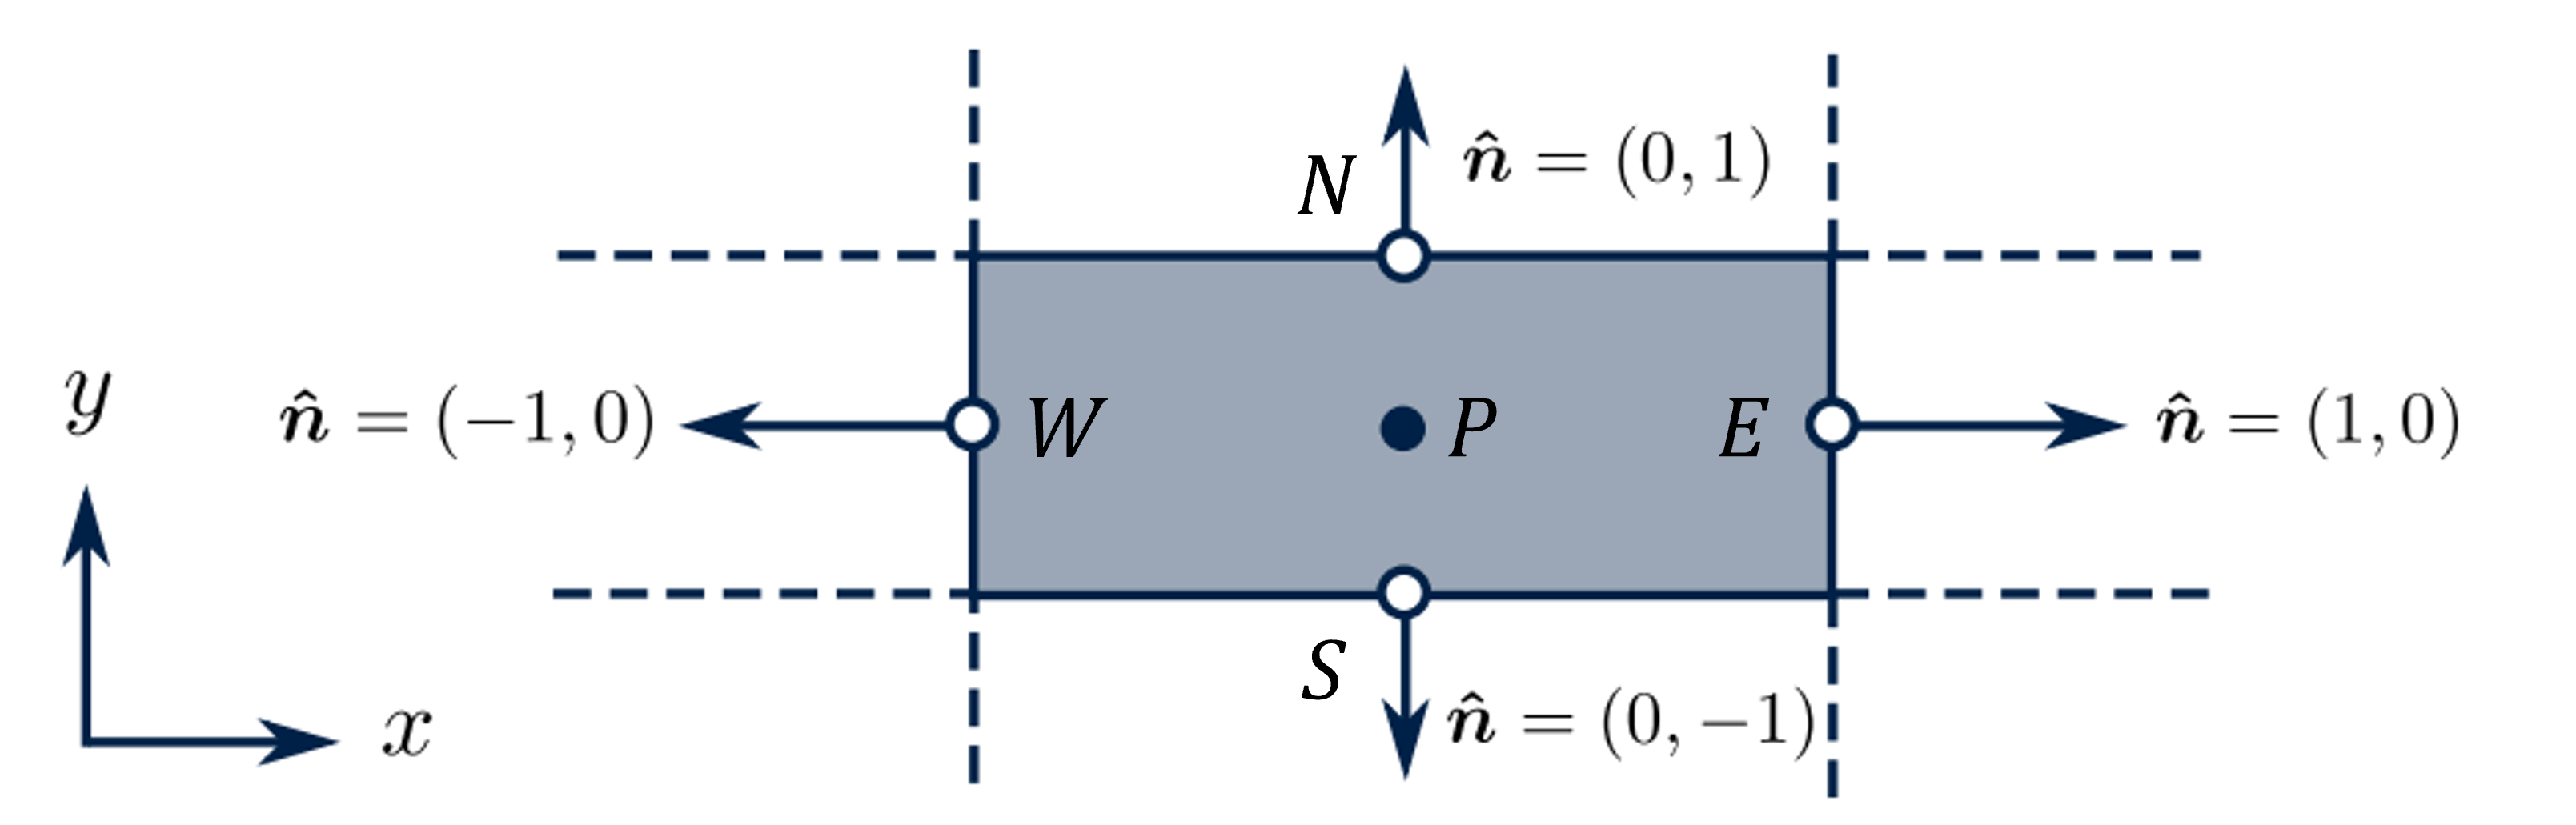
\includegraphics[scale=0.3]{normales_celda.png}
    \caption{ \centering{Vectores normales en direcciones norte ($N$), sur ($S$), este($E$) y oeste ($W$) para una celda 2D}}
    \label{norm_P}
\end{figure}

Teniendo lo anterior en mente y sabiendo que el término difusivo debe ser igual a la suma de los flujos en las fronteras con celdas vecinas ($ \int_S \left[ \Gamma \frac{\partial \phi}{\partial x_j} \hat{n}_j \right] dS = F_N + F_S + F_E + F_W $), pudo usarse el esquema de diferenciación central (CDS) para obtener:

\begin{equation*}
    \begin{split}
    F_e = \Gamma_e \frac{\phi_e-\phi_p}{x_E - x_P} \Delta y \quad ; \quad  F_w = -\Gamma_w \frac{\phi_p-\phi_w}{x_P - x_W} \Delta y \\
    \\[0.1cm]    
    F_n = \Gamma_n \frac{\phi_n-\phi_p}{y_N - y_P} \Delta x \quad ; \quad  F_s = -\Gamma_s \frac{\phi_p-\phi_s}{y_P - y_s} \Delta x        
    \end{split}    
\end{equation*}

La ecuación \eqref{int_S_eq1} fue reescrita de la siguiente manera:

\begin{multline}
    \frac{\Gamma_e \Delta y}{x_E-x_P} \phi_e + \frac{\Gamma_w \Delta y}{x_P-x_W} \phi_w + \frac{\Gamma_n \Delta x}{y_N-y_P} \phi_n \\
    + \frac{\Gamma_s \Delta x}{y_P-y_S} \phi_s - \frac{\Gamma_e \Delta y}{x_E-x_P} \phi_p - \frac{\Gamma_w \Delta y}{x_P-x_W} \phi_p \\
    - \frac{\Gamma_n \Delta x}{y_N-y_P} \phi_p - \frac{\Gamma_s \Delta x}{y_P-y_S} \phi_p + q_{\phi} \Delta x \Delta y  = 0
\end{multline}

Si se agrupa en coeficientes ($a_i$) para cada celda vecina, se reescribe la ecuación de la siguiente manera:

\begin{equation}
    a_E\phi_e + a_W\phi_w + a_N\phi_n + a_S\phi_s - \underbrace{(a_E+a_W+a_N+a_S)}_{\overset{a_P}{}} \phi_p = -q_{\phi} \Delta x \Delta y 
    \label{dis_int}
\end{equation}

La ecuación \eqref{dis_int} corresponde a la discretización general cuando una celda está rodeada por vecinas en todas las direcciones, es decir que se trata de la discretización para las \textbf{celdas internas}. 

Para las celdas que tienen una o más fronteras en su vecindad, se realizó la discretización correspondiente; a continuación se muestra para cada celda que tiene condiciones de frontera:

Para la \textbf{frontera norte}, en este caso tipo Neumann $(\partial T/\partial y=0)$, el coeficiente $a_N$ no aporta ni en las celdas vecinas ni en el coeficiente $a_P$ y el flujo establecido por la condición de frontera Neumann pasa a contribuir al lado conocido (en este caso es cero).

\begin{equation}
    a_E\phi_e + a_W\phi_w + a_S\phi_s - \underbrace{(a_E+a_W+a_S)}_{\overset{a_{P1}}{}} \phi_p = -q_{\phi} \Delta x \Delta y 
    \label{dis_N}
\end{equation}

En la \textbf{frontera sur} de tipo Dirichlet, el coeficinte $a_S$ no contribuye únicamente en las celdas vecinas pero si contribuye en el lado conocido.

\begin{equation}
    a_E\phi_e + a_W\phi_w + a_N\phi_n - \underbrace{(a_E+a_W+a_N+a_S)}_{\overset{a_{P}}{}} \phi_p = -q_{\phi} \Delta x \Delta y - a_S \phi_s 
    \label{dis_S}
\end{equation}

Para la \textbf{frontera este}, que también es tipo Dirichlet, ocurre algo análogo al caso de la frontera sur pero con el coeficiente $a_E$.

\begin{equation}
    a_W\phi_w + a_N\phi_n + a_S\phi_s - \underbrace{(a_E+a_W+a_N+a_S)}_{\overset{a_{P}}{}} \phi_p = -q_{\phi} \Delta x \Delta y - a_E \phi_e 
    \label{dis_E}
\end{equation}

Y de igual forma ocurre con la \textbf{frontera oeste} y el coeficiente $a_W$.

\begin{equation}
    a_E\phi_e + a_N\phi_n + a_S\phi_s - \underbrace{(a_E+a_W+a_N+a_S)}_{\overset{a_{P}}{}} \phi_p = -q_{\phi} \Delta x \Delta y - a_W\phi_w 
    \label{dis_W}
\end{equation}

En las celdas de las esquinas se tienen dos condiciones de frontera simultáneamente, y es por ello que sus efectos se combinan. Para el caso de la \textbf{celda noroeste} se obtuvo:

\begin{equation}
    a_E\phi_e + a_W\phi_w + a_S\phi_s - \underbrace{(a_E+a_W+a_S)}_{\overset{a_{P1}}{}} \phi_p = -q_{\phi} \Delta x \Delta y - a_W\phi_w
    \label{dis_NW}
\end{equation}

En el caso de la \textbf{celda noreste} se logró:

\begin{equation}
    a_W\phi_w + a_W\phi_w + a_S\phi_s - \underbrace{(a_E+a_W+a_S)}_{\overset{a_{P1}}{}} \phi_p = -q_{\phi} \Delta x \Delta y - a_E\phi_e
    \label{dis_NE}
\end{equation}

En las dos celdas inferiores hay dos condiciones Dirichlet aplicadas. Para el caso de la \textbf{celda suroeste} se llegó a:

\begin{equation}
    a_E\phi_e + a_N\phi_n - \underbrace{(a_E+a_W+a_N+a_S)}_{\overset{a_{P}}{}} \phi_p = -q_{\phi} \Delta x \Delta y - a_S\phi_s - a_W\phi_w 
    \label{dis_SW}
\end{equation}

Y finalmente para la \textbf{celda sureste}:

\begin{equation}
    a_W\phi_w + a_N\phi_n - \underbrace{(a_E+a_W+a_N+a_S)}_{\overset{a_{P}}{}} \phi_p = -q_{\phi} \Delta x \Delta y - a_S\phi_s - a_E\phi_e 
    \label{dis_SE}
\end{equation}

Así pues las ecuaciones \eqref{dis_int} a \eqref{dis_SE} corresponden a las discretizaciones para los nueve tipos de celdas que hay en el dominio computacional (internas, con una y con dos condiciones de frontera).

\section{Problema con solución analítica}
El problema con solución analítica se lleva a cabo en el mismo dominio, pero con condiciones de frontera diferentes, por lo que el código y la discretización cambia ligeramente.

$$
\begin{array}{|cc|}
    \hline \text { Frontera } & \text { Condición } \\
    \hline \text { Norte } & T=150^{\circ} \mathrm{C} \\
    \text { Sur } & T=15^{\circ} \mathrm{C} \\
    \text { Oeste } & T=15^{\circ} \mathrm{C} \\
    \text { Este } & T=15^{\circ} \mathrm{C} \\
    \hline \text { Conduct. } & \kappa=1 \\
    \text { Fuente } & B=0 \\
    \hline
\end{array}
$$

Este problema tiene la solución analítica dada por:

\begin{equation}
    T_{adimensional}(x,y) = \frac{2}{\pi}\cdot\sum_{n_{impar}}^\infty\frac{sinh(n\pi x/H)}{sinh(n\pi L/H)}\cdot sin(\frac{n\pi y}{H})
    \label{Sol_An_Ad}
\end{equation}

Para darle dimensiones de $^{\circ}\mathrm{C}$ se realizó el siguiente procedimiento:

\begin{equation}
    T(x,y)=\frac{T_{max}-T_{min}}{T_{adimensional}^{max}}\cdot T_{adimensional}(x,y) + T_{min}
    \label{Sol_An}
\end{equation}

\section{Método iterativo Gauss-Seidel}

Se escogió el método iterativo de Gauss-Seidel para la implementación en código ya que es intuitivo y fácil de escribir en código.

El método tiene el siguiente flujo para resolver el sistema matricial $[A][\phi]=[Q]$ con n incógnitas y n ecuaciones:

\begin{itemize}
	\item Hacer una estimación inicial para todas las incógnitas $\phi_{i}^0$.
	\item Resolver la primera ecuación del sistema de ecuaciones para obtener $\phi_{1}^1$.
	\item Resolver la segunda ecuación del sistema de ecuaciones teniendo en cuenta a $\phi_{1}^1$ para llegar a un valor de $\phi_{2}^1$
	\item Resolver la ecuación m-ésima teniendo en cuenta los nuevos valores de las $m-1$ incógnitas anteriores hasta completar las n ecuaciones.
	\item Calcular el residual de la siguiente forma:
	
	\begin{equation}
    	R=\sum^n|q_{\phi} - (a_P\phi_P + \sum_{j}^{vecinos} a_j\phi_j)|
    	\label{Res}
	\end{equation}
	
	\item Normalizar el residual dividiéndolo entre un flujo característico, así
	
	\begin{equation}
    	F=\sum^n|a_P\phi_P|
    	\label{Flujo_C}
	\end{equation}
	
	\item Comparando el residual normalizado con el criterio de convergencia $\epsilon$ se obtiene:
	
	\begin{equation}
    	\frac{R}{F}\leq\epsilon
    	\label{Res_norm}
	\end{equation}
	
	Si esta desigualdad es verdadera no realice más iteraciones pues el método convergió, si es falsa vuelva al segundo item de esta lista ya que el método no ha convergido.
\end{itemize}

Como métodos de salida del algoritmo se tiene:
\begin{itemize}
    \item Que el residual normalizado sea menor al criterio de convergencia.
    \item Que la diferencia entre el residual normalizado de la iteración anterior y el residual normalizado de la iteración actual sea menor que $1\times 10^{-9}$ y mayor que $0$.
    \item Que al haber pasado $1000$ iteraciones y si el residual normalizado de la iteración anterior es menor que el de la iteración actual.
    
Dado que se decidió utilizar los métodos de salida del método anteriormente mencionados no se usó ninguna librería en particular para el mismo.
\end{itemize}

\section{Estado actual de los Códigos}
Al momento se tienen completos lo códigos del problema con solución analítica y del problema de interés con solución en serie en los cuales se utiliza la librería \textbf{Vector}.

Por otra parte, en el caso del problema de interés paralelizado en las funciones que son objetivo de la paralelización se utiliza la librería \textbf{Eigen} y para obtener \textit{CPU time} y \textit{Wall clock time} se utilizan la función \textbf{std::clock\_t} y la librería \textbf{Chrono} respectivamente. No obstante, hace falta implementar las líneas de código que contienen \textit{\#pragma}.

Al momento, los objetivos se mantienen puesto que sólo hace falta implementar las líneas de paralelización.

\section{Resultados}
\subsection{Caso con solución analítica}

En esta parte se van a mostrar los resultados obtenidos de las soluciones analítica y numérica del problema de conducción de calor en la placa rectangular.

\begin{figure}[H]
    \centering
    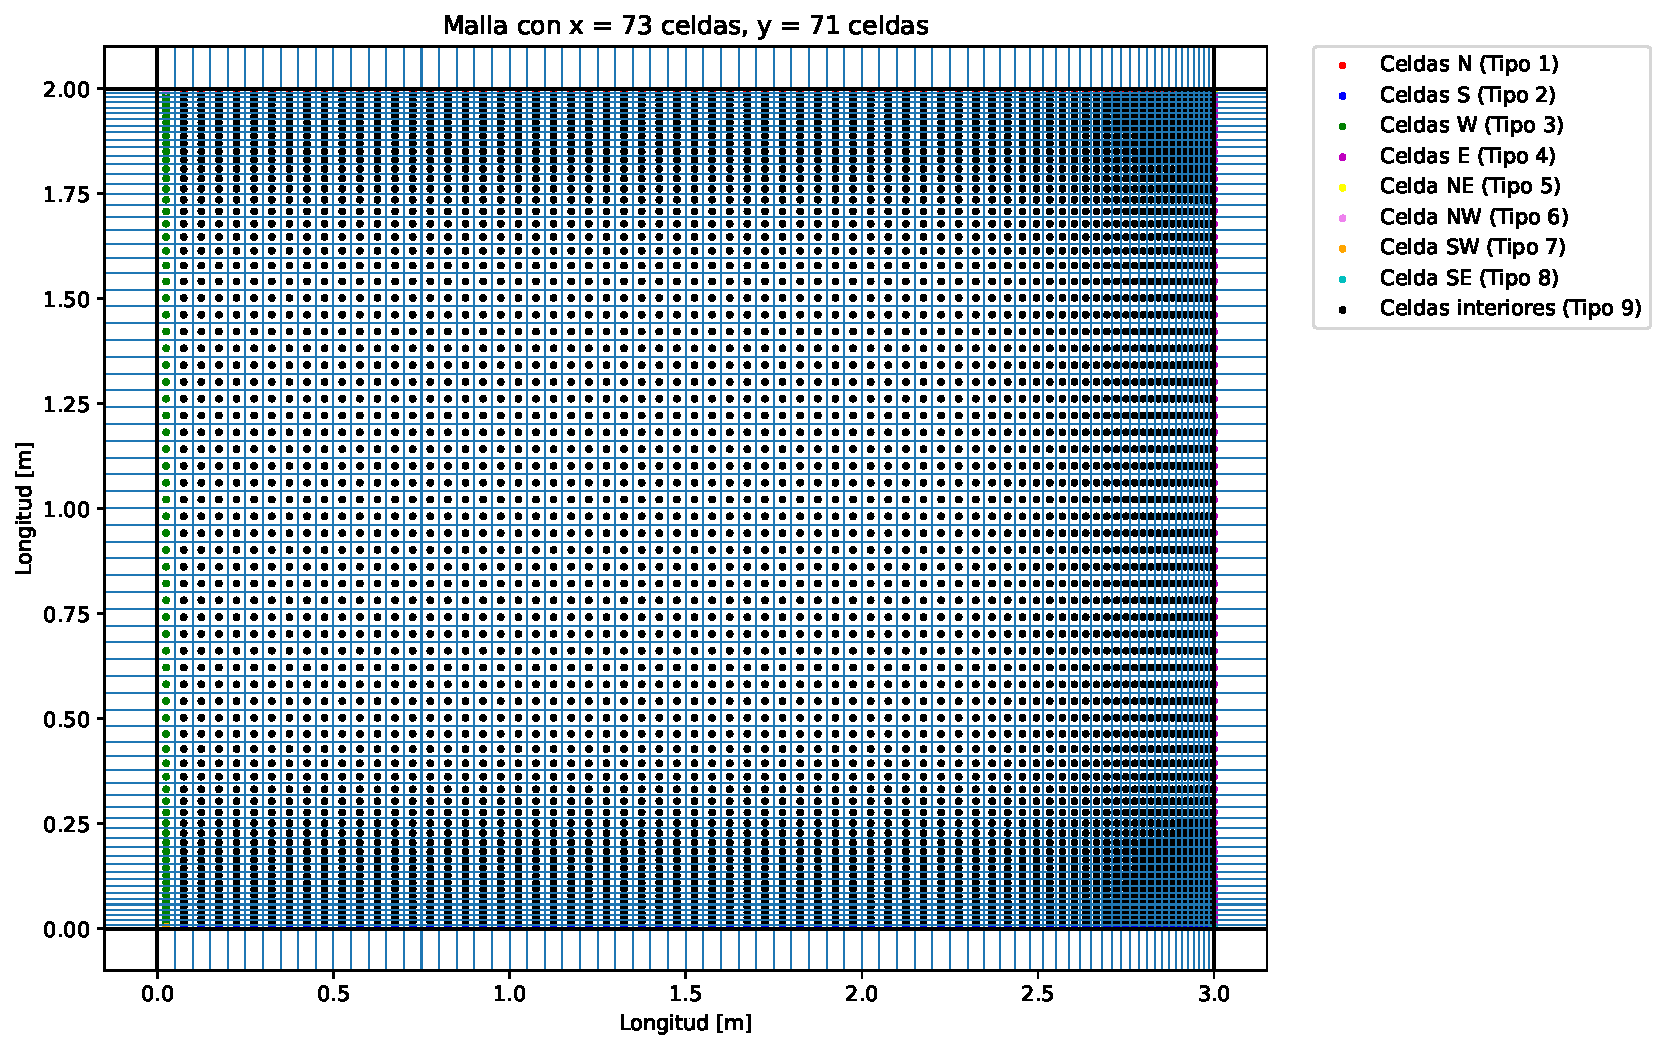
\includegraphics[scale=0.25]{Caso_analitico/Malla.pdf}
    \caption{ \centering{Malla utilizada para el caso con solución analítica}}
    \label{Malla_An_num}
\end{figure}

En la figura \ref{Malla_An_num} se puede ver la malla utilizada para resolver este problema, se puede apreciar que la malla tiene un refinamiento hacia la frontera este, la frontera norte y sur, ya que allí en las esquinas nor-este y sur-este son los lugares donde se concentran los mayores gradientes de temperatura y se acumulan las líneas isotermas.

\begin{figure}[H]
    \centering
    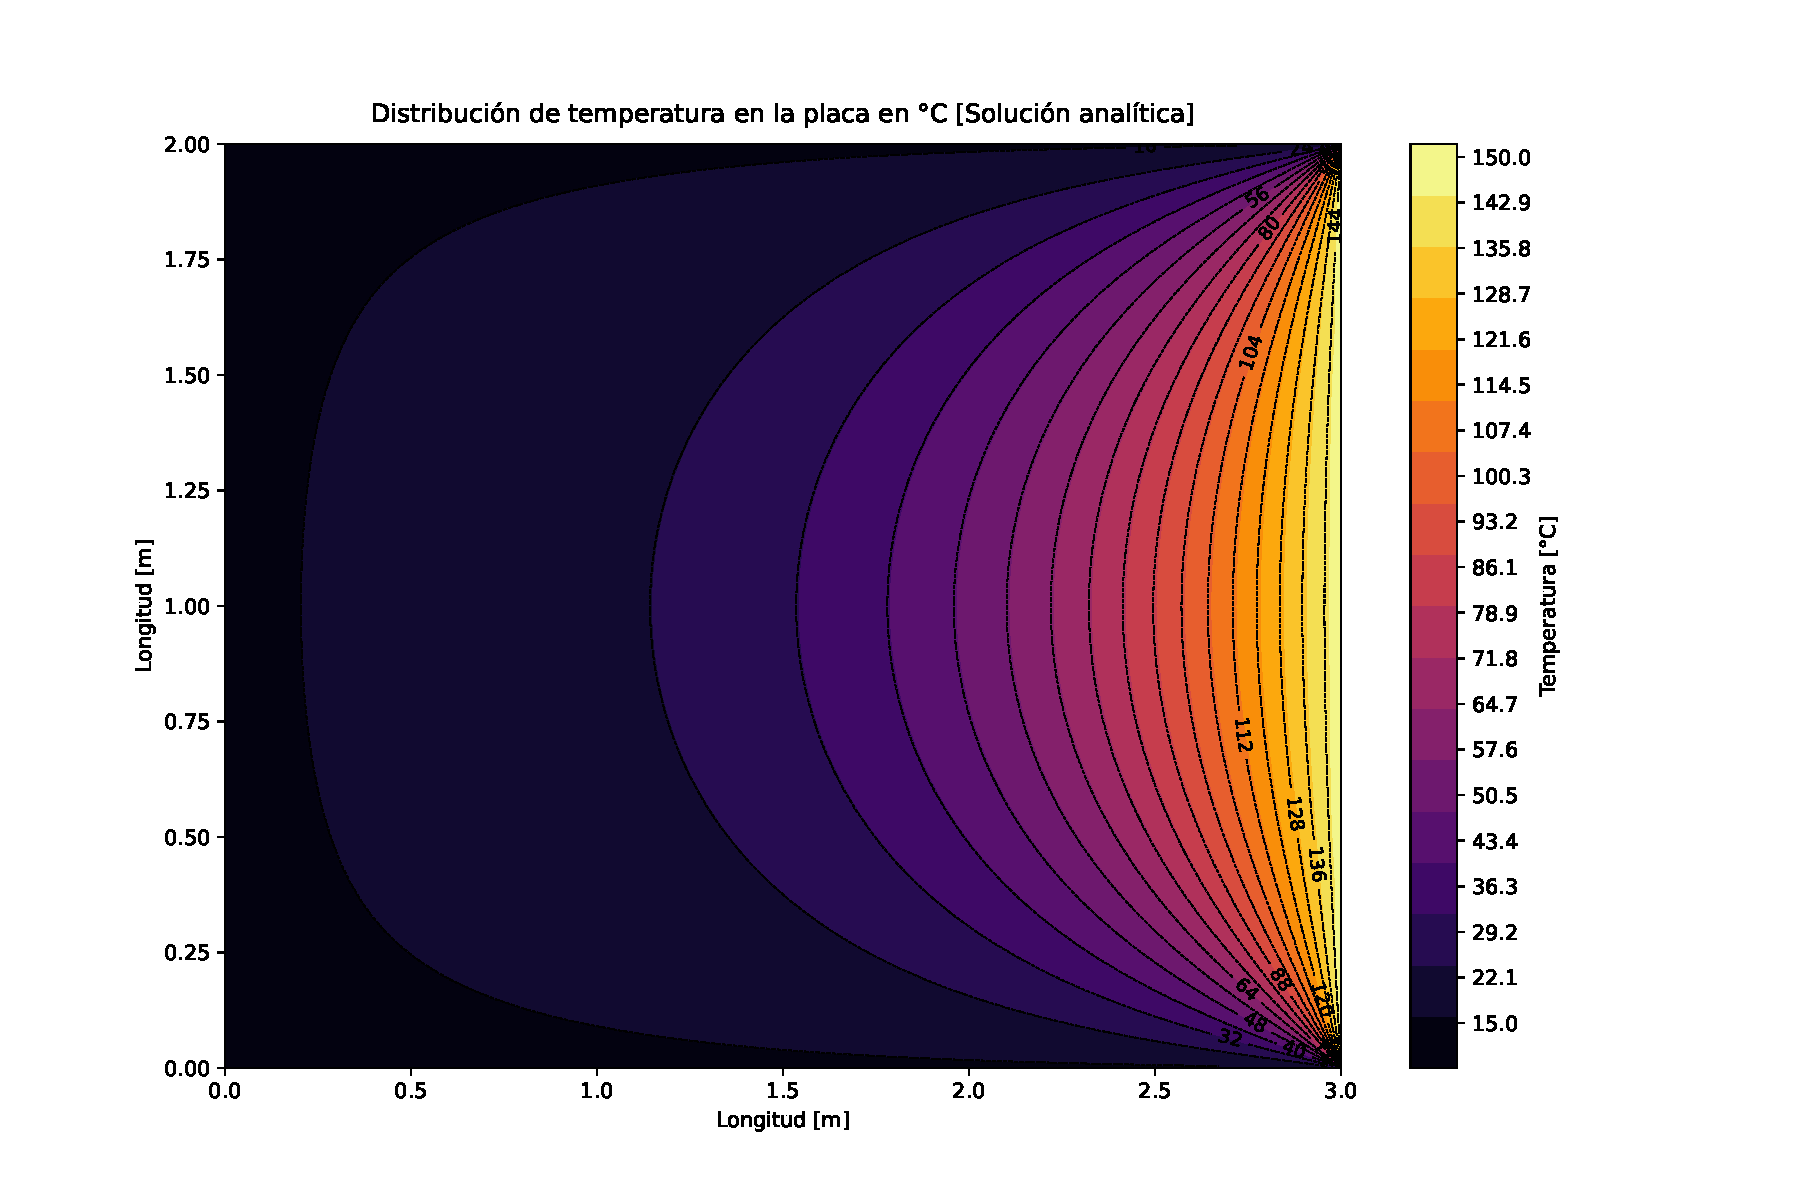
\includegraphics[scale=0.25]{Caso_analitico/Dist_T_An.pdf}
    \caption{ \centering{Distribución de temperatura con la solución analítica}}
    \label{T_Sol_An}
\end{figure}

Ahora bien, en la imagen \ref{T_Sol_An} se ve la distribución de temperatura en la placa con la solución analítica; no obstante, hay que ser consiente de que esta tiene el error de truncamiento debido a que no se podía tener los infinitos términos de la serie, por lo que sólo se usaron $75$ términos.

\begin{figure}[H]
    \centering
    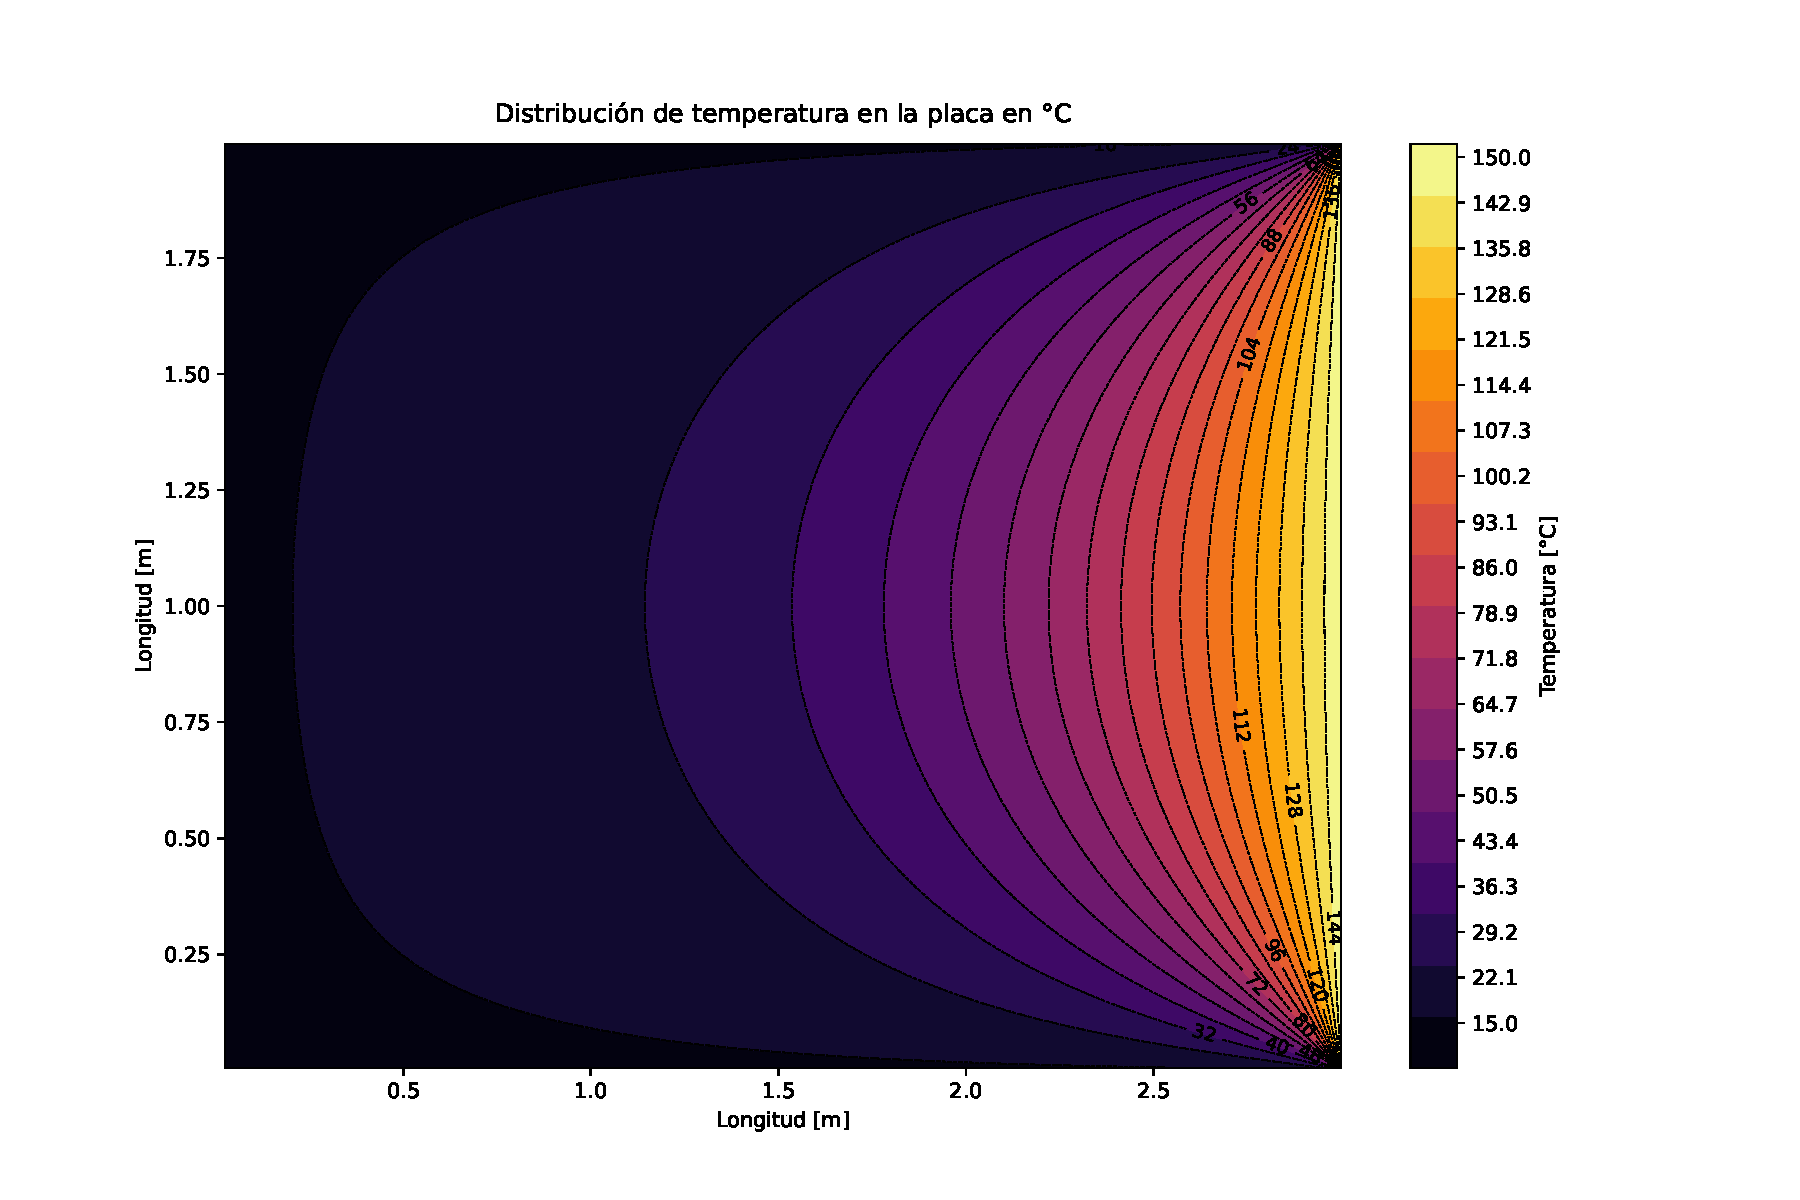
\includegraphics[scale=0.25]{Caso_analitico/Dist_T.pdf}
    \caption{ \centering{Distribución de temperatura con la solución numérica}}
    \label{T_Sol_An_num}
\end{figure}

Por otra parte, en la figura \ref{T_Sol_An_num} se puede observar la distribución de temperatura en la placa con la solución numérica.

\begin{figure}[H]
    \centering
    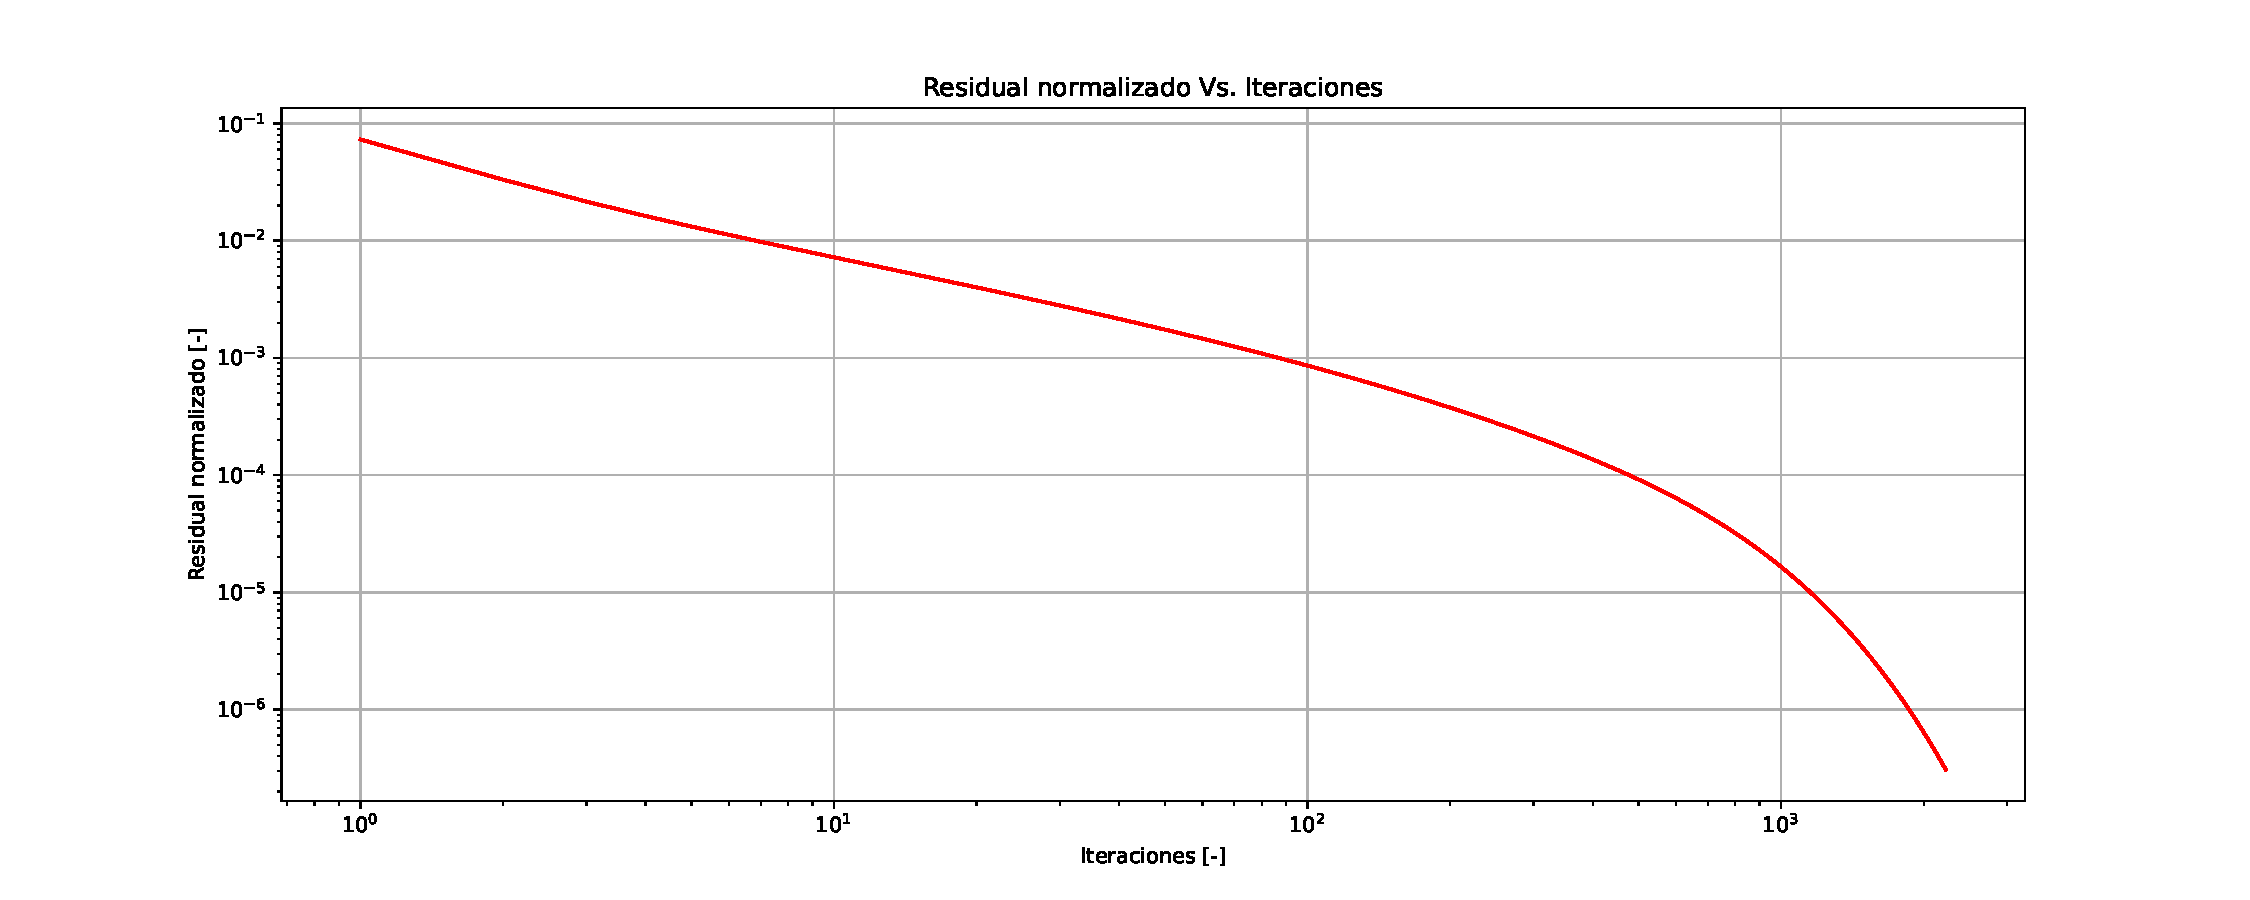
\includegraphics[scale=0.2]{Caso_analitico/Residuales.pdf}
    \caption{ \centering{Residual normalizado de la solución numérica del caso con solución analítica}}
    \label{Res_An_num}
\end{figure}

En este problema, el residual normalizado tuvo el comportamiento expuesto en la figura \ref{Res_An_num}, alcanzando las $2226$ iteraciones con un residual normalizado de $3.081\cdot 10^{-7}$. Por lo tanto, el problema no alcanzó el criterio de convergencia, pero la curva llegó a cambiar menos que $1\cdot 10^{-9}$ y salió del método iterativo.

\subsection{Caso de interés}

\begin{figure}[H]
    \centering
    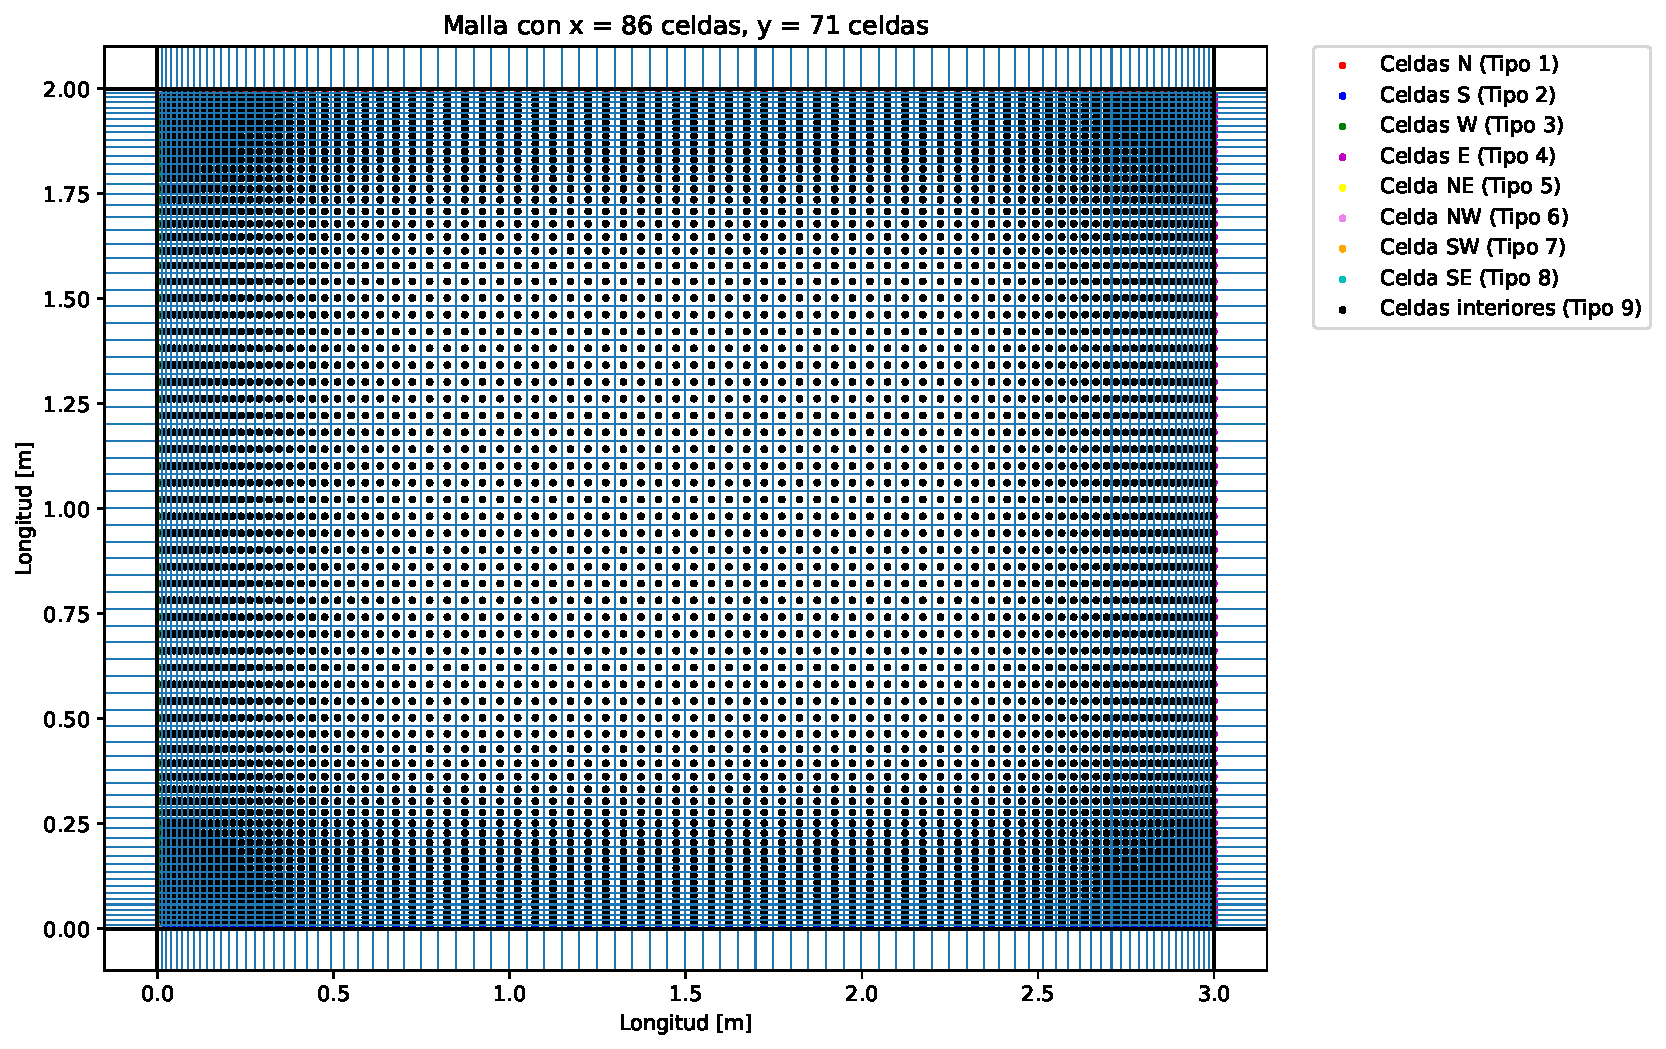
\includegraphics[scale=0.25]{Caso_interes/Malla.pdf}
    \caption{ \centering{Malla utilizada para el caso de interés}}
    \label{Malla_int}
\end{figure}

En la figura \ref{Malla_int} se puede apreciar la malla utilizada para resolver este caso. Es posible ver el refinamiento que hay hacia las esquinas inferiores y en general en la frontera sur, ya que en esa región es donde está la frontera de tipo Dirchlet que cambia con la función $sin(x)$.

\begin{figure}[H]
    \centering
    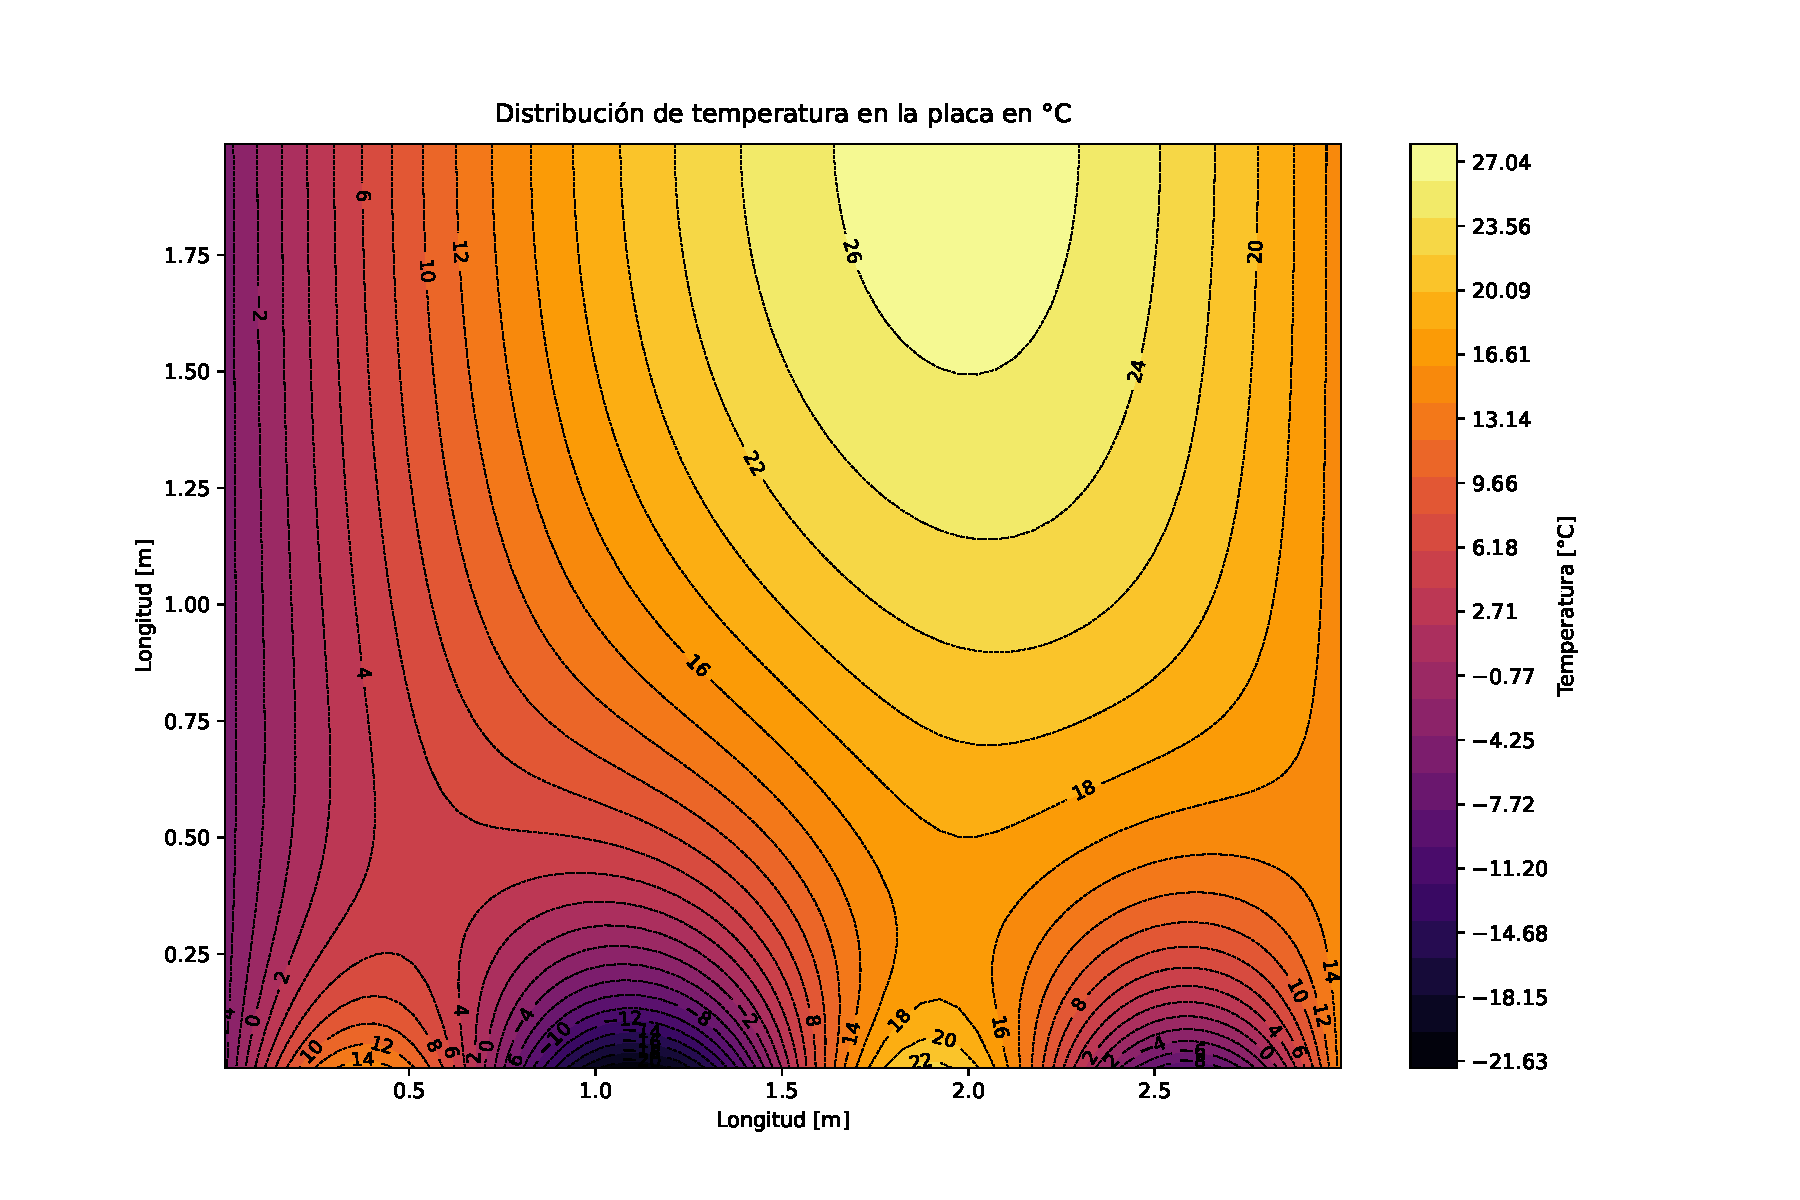
\includegraphics[scale=0.25]{Caso_interes/Dist_T.pdf}
    \caption{ \centering{Distribución de temperatura con la solución numérica}}
    \label{T_int}
\end{figure}

Así pues, en la figura \ref{T_int} se puede observar la distribución de temperatura en la placa del problema de interés. Se aprecia cómo se aglomeran las isotermas en la frontera sur y las esquinas sur-este y sur-oeste.

\begin{figure}[H]
    \centering
    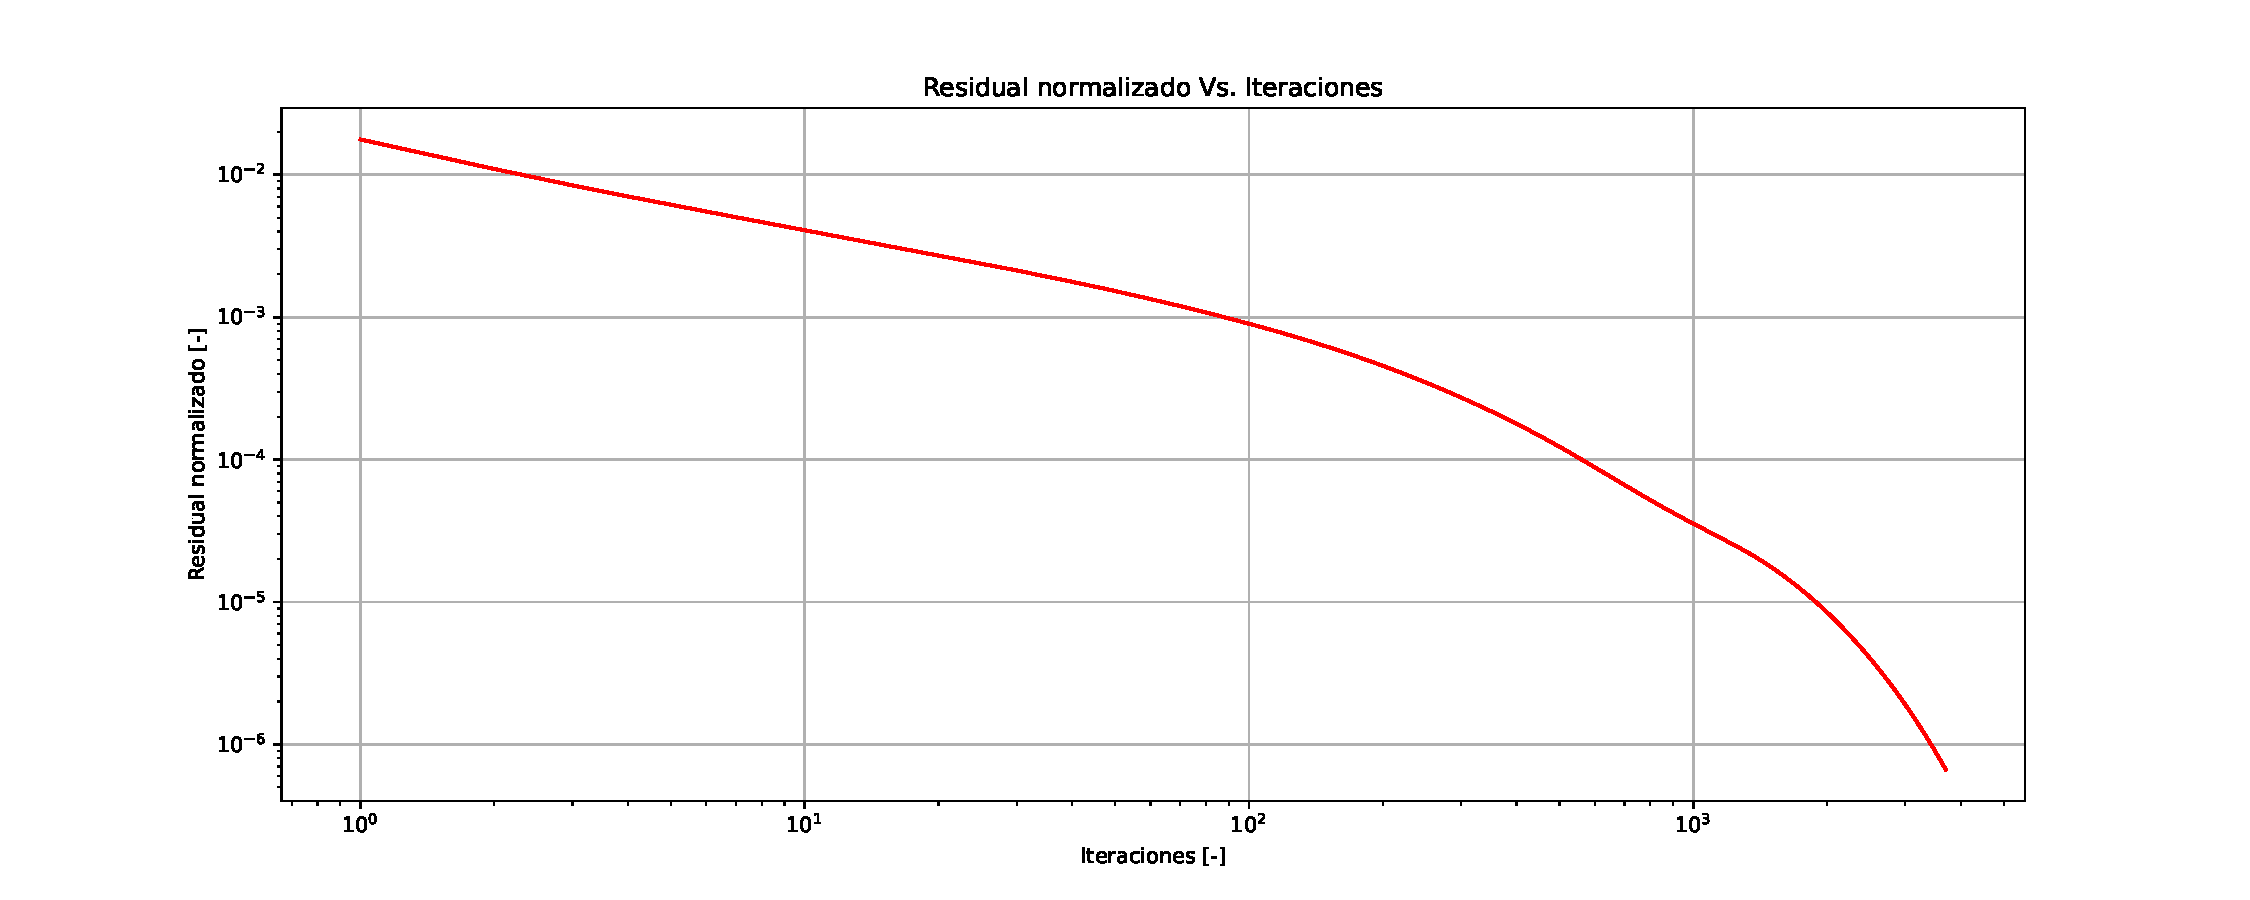
\includegraphics[scale=0.2]{Caso_interes/Residuales.pdf}
    \caption{ \centering{Residual normalizado de la solución numérica del caso de interés}}
    \label{Res_int}
\end{figure}

En este caso, el residual normalizado se comportó de la forma en que muestra la figura \ref{Res_int}, alcanzando las $3701$ iteraciones con un residual normalizado de $6.667\cdot 10^{-7}$. Entonces, la curva llegó a tener una variación menor que $1\cdot 10^{-9}$, por lo que salió del ciclo \textit{while} de la función del método iterativo de Gauss-Seidel.

\subsection{Caso de interés paralelizado}

Las pruebas en este caso se han llevado a cabo con una malla de $25$ celdas en x y $20$ celdas en y.

\begin{center}
  \begin{tabular}{|c|c|c|}
    \hline
    \multicolumn{3}{|c|}{Tiempos obtenidos para la función Malla.cpp} \\
    \hline
    Num Threads & Wall clock time [s] & CPU time [s] \\
    \hline
    1 & 0.000298705 & 0.000298 \\
    \hline
    2 & 0.000283928 & 0.000287 \\
    \hline
    3 & 0.000289217 & 0.000292 \\
    \hline
    4 & 0.00027976 & 0.000282 \\
    \hline
    5 & 0.000278377 & 0.000282 \\
    \hline
    6 & 0.000275903 & 0.000279 \\
    \hline
    7 & 0.000277606 & 0.00028 \\
    \hline
    8 & 0.000272146 & 0.000275 \\
    \hline
    9 & 0.000288416 & 0.000291 \\
    \hline
    10 & 0.000276424 & 0.000279 \\
    \hline
    11 & 0.000305148 & 0.00031 \\
    \hline
    12 & 0.000282675 & 0.000285 \\
    \hline
    13 & 0.000277786 & 0.00028 \\
    \hline
    14 & 0.000291212 & 0.000295 \\
    \hline
    15 & 0.000325246 & 0.000324 \\
    \hline
    16 & 0.000289238 & 0.000292 \\
    \hline
  \end{tabular}
\end{center}

\begin{center}
  \begin{tabular}{|c|c|c|}
    \hline
    \multicolumn{3}{|c|}{Tiempos obtenidos para la función Procesamiento.cpp} \\
    \hline
    Num Threads & Wall clock time [s] & CPU time [s] \\
    \hline
    1 & 2.19908 & 2.19757 \\
    \hline
    2 & 2.20235 & 2.20111 \\
    \hline
    3 & 2.15537 & 2.1542 \\
    \hline
    4 & 2.16737 & 2.16602 \\
    \hline
    5 & 2.22489 & 2.22368 \\
    \hline
    6 & 2.18364 & 2.18222 \\
    \hline
    7 & 2.19653 & 2.19536 \\
    \hline
    8 & 2.20293 & 2.20141 \\
    \hline
    9 & 2.19433 & 2.193 \\
    \hline
    10 & 2.22594 & 2.22479 \\
    \hline
    11 & 2.21002 & 2.20844 \\
    \hline
    12 & 2.18639 & 2.18527 \\
    \hline
    13 & 2.20686 & 2.2055 \\
    \hline
    14 & 2.21453 & 2.21278 \\
    \hline
    15 & 2.16336 & 2.16197 \\
    \hline
    16 & 2.16896 & 2.16782 \\
    \hline
  \end{tabular}
\end{center}
  
En las tablas anteriores se puede apreciar que el proceso de paralelización no funciona en el momento, lo cual muestra que faltan los comandos \textit{\#pragma}.

\newpage

\begin{thebibliography}{}
\bibitem{C1} Benavides, A. \textit{CFD Finite Volume Method}, Computational Fluid Dynamics, 2023.
\bibitem{C2} Versteeg, H \& Malalasekera, W. \textit{An Introduction to Computational Fluid Dynamics}, Second edition, 2007.
\bibitem{C3} Wimshurst, A. \textit{Lecture Notes, Computational Fluid Dynamics}, Fundamentals Course 2, 2020.
\bibitem{C4} Pletcher, R. H., Tannehill, J. C., \& Anderson, D. \textit{Computational fluid mechanics and heat transfer}, 2012.
\bibitem{C5} Minkowycz, W. J., Sparrow, E. M., Schneider, G. E., \& Pletcher, R. H. \textit{Handbook of numerical heat transfer}, 1988.
\bibitem{C6} “C++ variables de tipo vector,” Inicio. [Online]. Available: \url{https://aprende.olimpiada-informatica.org/cpp-vector}.
\bibitem{C7} “2D vector in C++ with user defined size,” GeeksforGeeks, 10-Jan-2023. [Online]. Available: \url{https://www.geeksforgeeks.org/2d-vector-in-cpp-with-user-defined-size/}. 
\bibitem{C8} D. Krishna, “Different ways to remove elements from vector in C++ STL,” OpenGenus IQ: Computing Expertise \&amp; Legacy, 26-Oct-2019. [Online]. Available: \url{https://iq.opengenus.org/ways-to-remove-elements-from-vector-cpp/}. 
\bibitem{C9} “Reading in .DAT file, line by line,” C++ forum. [Online]. Available: \url{https://cplusplus.com/forum/beginner/117331/}.
\bibitem{C10} “Modules and header files,” Eigen. [Online]. Available: \url{https://eigen.tuxfamily.org/dox/group\_\_QuickRefPage.html}.
\bibitem{C11} Barney, B, “OpenMP,” LLNL HPC Tutorials. [Online]. Available: \url{https://hpc-tutorials.llnl.gov/openmp/}. 
\end{thebibliography}

\end{document}
